\section{Theoretische Grundlagen} \label{sec:TheoretischeGrundlagen}

\subsection{EMI-Filter} \label{subsec:emifilter}
Das vorgegebene EMI-Filter muss bezüglich der Einfügungsverluste (insertion loss) untersucht werden. Die Einfügunsverluste hängen vom Gesamtrauschen der Schaltung ab. Es wird ein Ansatz verwendet, der in der Praxis weit verbreitet ist, bei welchem das Gesamtrauschen in zwei Komponenten unterteilt wird. Man spricht vom Gegen-(=Differential Mode=DM) und Gleichtaktrauschen (=Common Mode=CM). Anhand der vorgegebenen CM- und DM-Äquivalenten Schaltungen werden die Einfügungsverluste in Funktion der Frequenz berechnet. Die Berechnungen decken einen Bereich von 0 bis 30MHz ab.

Die Einfügungsverluste sind wie folgt definiert: 

\begin{equation}
\left\lvert IL\right\rvert =\left\lvert H(j\omega) \right\rvert = 20*log(\frac{ \left\lvert U_{20} \right\rvert }{ \left\lvert U_2 \right\rvert })
\end{equation}
In der Definition kann das Spannungsverhältnis durch den Streuparameter (S-Parameter) S\textsubscript{21} ersetzt werden. Dieser Parameter beschreibt den Transmissionsgrad des Filters. Die Einfügungsverluste wären auch mit dem Verhältnis von eingehende zu abegegebene Leistung zu berechnen, jedoch eignet sich diese Methode mehr beim messtechnischen bestimmen der Einfügungsverluste. 
\begin{equation}
\left\lvert IL\right\rvert = 20*log (\left\lvert S_{21} \right\rvert)
\end{equation}
Folgende Schaltungen stellen die CM- und DM-Äquivalenten Schaltungen. Da die Berechnungen in einem Bereich von bis zu 30 MHz gemacht werden, ist es notwendig die parasitären Parameter von Spule und Kondensator miteinzubeziehen.
\subsection{Schaltungen} \label{subsec:schaltungen}
CM:
\begin{figure}[H]
	\centering
	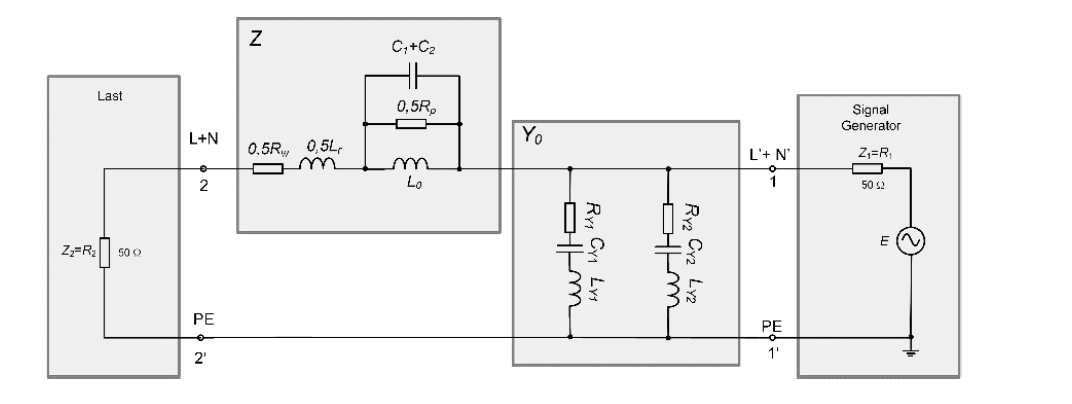
\includegraphics[width=15cm]{CM_ElectricalCircuit.png}
	\caption{CM-Schaltungäquvalent}
	\label{fig:CM-Schaltungäquvalent}
\end{figure}
DM:
\begin{figure}[H]
	\centering
	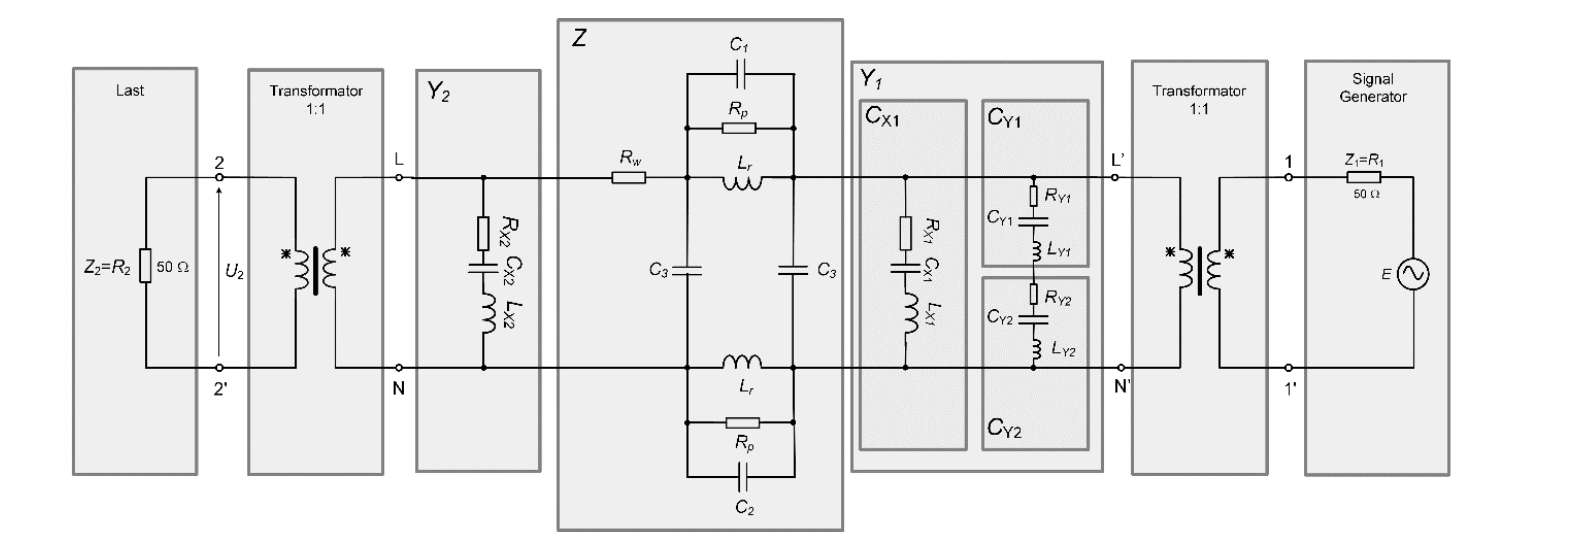
\includegraphics[width=15cm]{DM_ElectricalCircuit.png}
	\caption{DM-Schaltungsäquvalent}
	\label{fig:DM-Schaltungsäquvalent}
\end{figure}

\subsection{Vorgehen} \label{subsec:vorgehen}
Die Einfügungsverluste werden analytisch ermittelt. Im ersten Schritt werden die Berechnungen in MATLAB gemacht. Somit können die Funktionen  geplottet werden. Diese Plots werden dann mit Simulationen in MPLAB Mindi verglichen um festzustellen ob diese korrekt sind. Die vollständigen und korrekten Berechnungen können somit in Java implementiert werden. Um die Einfügungsverluste bestimmen zu können, wird das Model der 2-Tore verwendet. Einzelne Schaltungsteile werden in ABCD-Matrixen abgebildet, welche dann durch Kaskadierung der einzelnen ABCD-Matrixen zusammengeführt werden. Die Einfügungsverluste werden aus den S-Parameter abgeleitet, welche direkt aus der ABCD-Matrix berechnet werden.
Der S-Parameter S\textsubscript{21} gibt den Transmissionsgrad der Wellen an, die vom Tor 1 zum Tor2 übertragen wird. Die S-Parameter sind abhängig von den Bezugswiderständen (Innenwiderstand der Quelle sowie Lastwiderstand). In unserem Fall sind die Bezugswiderstände mit 50Ohm gegeben.

\newpage
\subsection{Berechnungsbeispiel} \label{subsec:beispiel}
Folgender Abschnitt zeigt auf, wie die Einfügungsverluste ermittelt werden. Als Beispielschaltung wird das CM-Schaltungsäquivalent verwendet. Die Schaltung beinhaltet eine Queradmittanz und eine Längsimpedanz, welche in Schritt 1 zusammengefasst werden. Im Schritt 2 werden diese dann in die ABCD-Matrixen(Kettenmatrixen) eingesetzt. Durch kaskadieren der einzelnen Kettenmatrixen wird in Schritt 3 die Kettenmatrix der kompletten Schaltung erstellt. Diese Kettenmatrix kann nun zusammen mit dem Bezugswiderstand in die Definition des Streuparameters S21 eingesetzt werden (Schritt 4).

\begin{figure}[H]
	\centering
	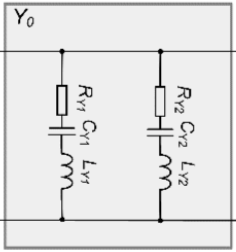
\includegraphics[width=5cm]{CM_Admittanz.png}
	\caption{CM-Admittanz}
	\label{fig:CM-Admittanz}
\end{figure}
\begin{figure}[H]
	\centering
	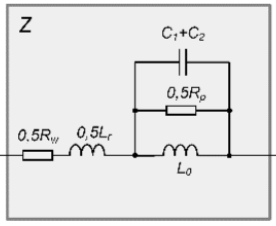
\includegraphics[width=5cm]{CM_Impedanz.png}
	\caption{CM-Impedanz}
	\label{fig:CM-Impedanz}
\end{figure}
Schritt 1: Berechnen der Längsimpedanz Z und der Queradmittanz Y0.
Für die Querimpedanz Y0 ergibt sich die Formel
\begin{equation}
Y_0 = \frac{ 1 }{R_{y1} + \frac{1}{j*\omega*C_{y1}}+j*\omega*L_{y1}} +\frac{ 1 }{R_{y2} + \frac{1}{j*\omega*C_{y2}}+j*\omega*L_{y2}}
\end{equation}

Für die Längsimpedanz ergibt sich folgende Formel
\begin{equation}
Z = 0.5*R_w+j*\omega*L_r+\frac{ 1 }{ \frac{1}{0.5*R_p}+j*\omega*L_r*(C_1+C_2)+\frac{1}{j*\omega*L_0} }
\end{equation}


Schritt 2: Erstellen der ABCD-Matrixen.

Somit ergeben sich die ABCD-Matrixen wie folgt
\begin{equation}
A_1 =
\begin{matrix}
1 & 0\\ Y&1 
\end{matrix}
\end{equation}
\begin{equation}
A_2 =
\begin{matrix}
1 & Z\\ 0&1 
\end{matrix}
\end{equation}

Schritt 3: Gesamt-Kettenmatrix bilden
Die ABCD-Matrixen haben den Vorteil, dass man sie sehr unkompliziert kaskadieren kann indem man das Produkt bildet.
\begin{equation}
A = A_1*A_2 = A_2 = \begin{matrix}
1 & 0\\ Y&1 
\end{matrix} * 
\begin{matrix}
1 & Z\\ 0&1 
\end{matrix} 
\end{equation}

Schritt 4: S21 Parameter bilden.

Der S21 Parameter ist wie folgt definiert.

\begin{equation}
S_{21} = \frac{2}{A_{11}+\frac{A{12}}{R_w}+A_{21}*R_w+A_{22}}
\end{equation}

Somit sind alle gesuchten Werte gegeben und der S21 Parameter wird durch einsetzen der Werte gebildet.

Schritt 5: Einfügungsverluste bilden

Durch einsetzen des Streuparameters S21 in die Definition der Einfügunsverluste lassen sich diese Darstellen. Folgende Grafik zeigt die Berechnungen in MATLAB (Mitte) im Direktvergleich mit der Grafik aus der Aufgabenstellung(Links) sowie die Simulation in MPLAB Mindi (Rechts). Die Differenzen lassen sich dadurch erklären, dass in der Aufgabenstellung die Werte der Bauelemente nicht gegeben sind.
\begin{figure}[H]
	\centering
	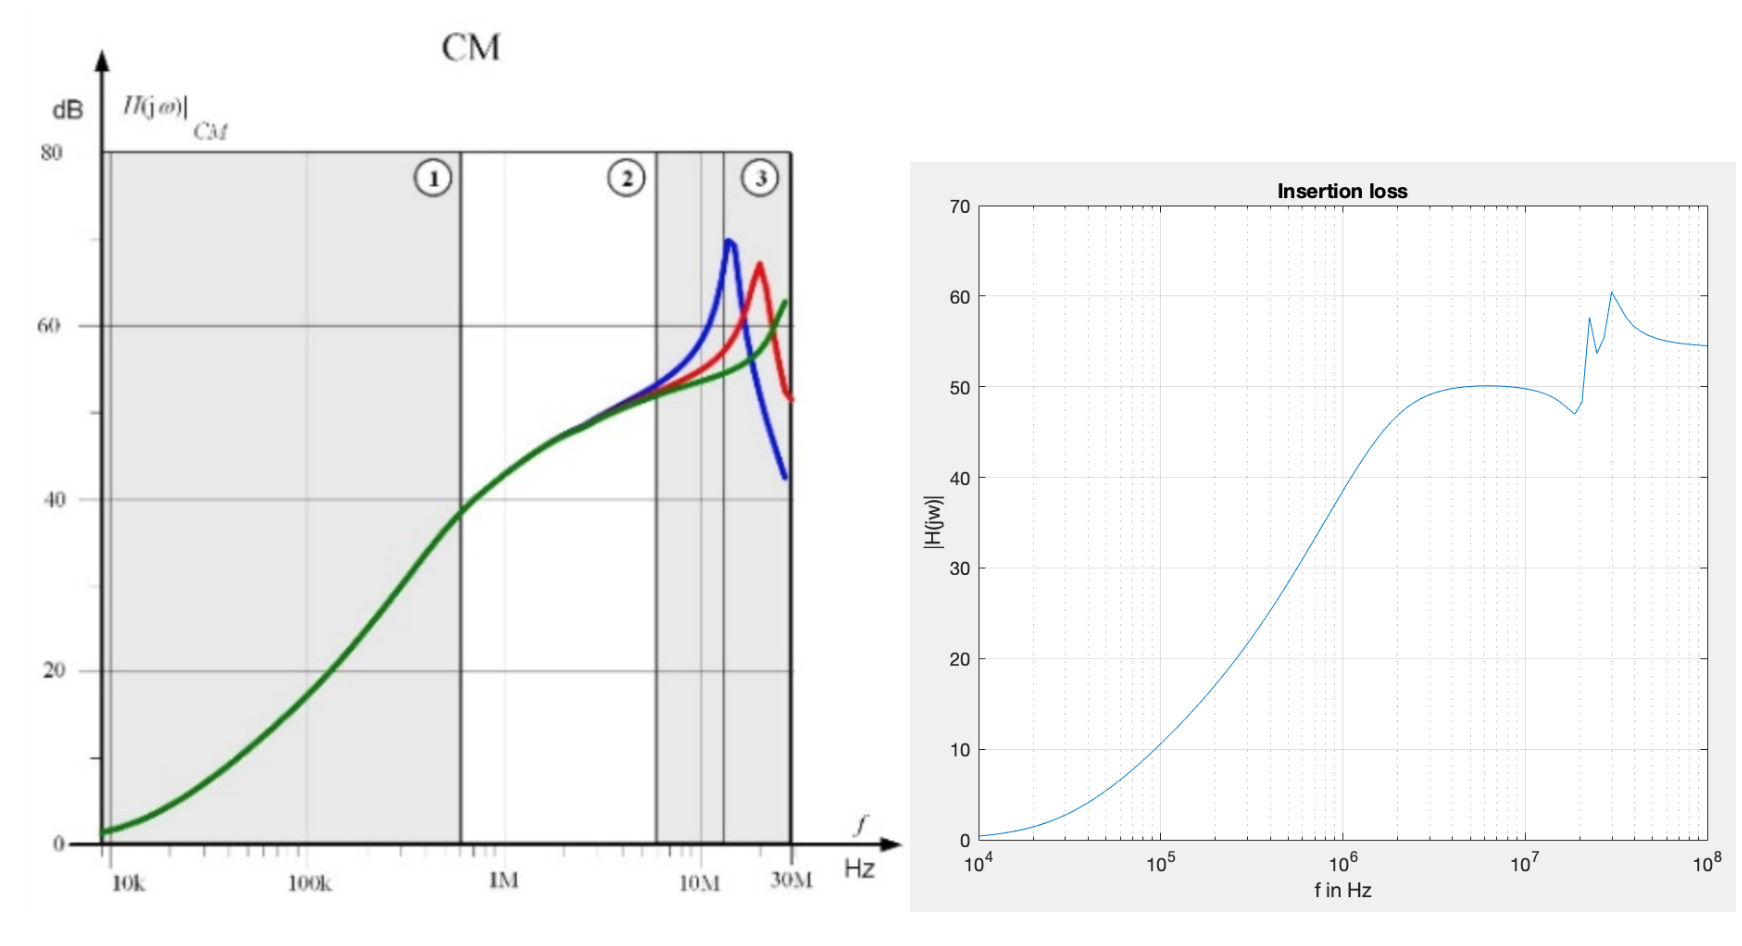
\includegraphics[width=15cm]{CM_vergleich.png}
	\caption{Vergleich}
	\label{fig:Vergleich Berechnung Simulation}
\end{figure}
